\section{Kapacitet} \label{kap}
% Skriv ift kapacitet (ift sengepladser, persona - hvilken betydning har hhv. 95 \% kapacitet mod 105 \%)
Kapacitetudnyttelsen er forholdet mellem aktivitet og kapacitet. Aktivitet omhandler patient og kontakt. Herunder består kontakt af forundersøgelse, behandling og kontrol. Kapacitet omfatter antallet af personale, udstyr og rum. Personalet består af læger, sygeplejersker og sekretærer. Udstyret beskriver de nødvendige maskiner samt antallet af rum, der opbevarer udstyret. Den samlede kapacitetsudnyttelse er defineret ud fra, at der produceres mest muligt for de investerede ressourcer.\cite{Company2013} En illustration af kapacitetsudnyttelse fremgår af \figref{kapacitet}.

\begin{figure}[H]
	\flushleft 
	\centering
	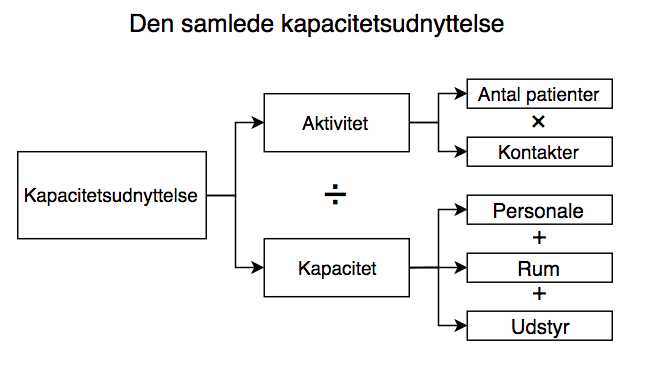
\includegraphics[scale=0.6]{figures/Kapacitetsudnyttelse.png}
	\flushleft
	\caption{\textit{Den samlede kapacitetsudnyttelse, som er definineret ved forholdet mellem aktivitet og kapacitet. Aktivitet omfatter antallet af patienter og kontakter. Kapacitet omfatter personale, rum og udstyr.\cite{Company2013}}}
	\label{kapacitet}
\end{figure}

\noindent
Ud fra \figref{kapacitet} fremgår det, at kapacitetsudnyttelse er forholdet mellem aktivitet  og kapacitet. Dertil ses aktivitet som antal patienter multipliceret med kontakter og kapaciteten bestående af personale, rum og udstyr lagt sammen. Antallet af patienter, som fremgår af \figref{kapacitet}, beskriver ligeledes belægning på hospitalets afdelinger. \cite{Company2013} 

Belægning er defineret ud fra antallet af patienter, der er normeret til på en afdeling \cite{Heidmann2014}. Når en $100~\%$ belægning opnås, svarer dette til, at alle sengepladser på en afdeling er taget i brug. Ved en belægning på over $100~\%$ betyder det, at der er flere patienter end afdelingen er normeret til, hvilket vil sige, at afdelingen yder mere end der er kapacitet til. Ud fra \figref{kapacitet} vil dette betyde at der ikke er ligevægt mellem aktivitet og kapacitet, hvilket forårsager kapacitetsmangel på afdelingen. Det kan derfor være nødvendigt at tilkalde ekstra personale for at opnå en balance i kapaciteten.\cite{Pauly1986}
Hvis der derimod er en belægning på under $100~\%$ er der omvendt færre patienter end afdelingen er normeret til, dette betyder, at der er flere sengepladser end patienter. Dette fører ligeledes til ubalance i kapacitetsudnyttelsen som vist på \figref{kapacitet}. I denne situation er der mere personale end nødvendigt til at varetage de enkelte patienter, hvilket betyder, at der ikke er fuld udnyttelse af personalet.\cite{Pauly1986} 
Det anses herved vigtigt, at der er balance mellem aktivitet og kapacitet, således de investerede ressourcerne udnyttes optimalt. Det ønskes derfor for afdelingerne, at opnå en kapacitetsudnyttelse på 100\%.   

\subsection{Ortopædkirurgisk afdeling}
Udnyttelsen af kapaciteten afhænger ligeledes af det budget som afdelingen har til rådighed. Dette beløb udregnes ud fra diagnoserelaterede grupper (DRG) systemet. Systemet anvendes til at analysere omkostninger og aktivitet på et hospital.\cite{DRG2016} Ortopædkirurgisk afdeling har et budget på $700.872.744$ kr, som svarer til 17,2 \% af det samlede budget for alle afdelinger på Aalborg Universitetshospital. Det samlede DRG for afdelingerne på Aalborg Universitetshospital er illusteret af \figref{DRG_budget}.\cite{Rasmussen2016}
Størstedelen af budgettet anvendes til personale- og patient udgifter, som svarer til hhv. 60 \% og 32 \%. Det resterende budget anvendes til bygninger, it, apparatur, inventar samt drift og service \cite{Nøgletal2016}. 

% \begin{figure}[H]
% \flushleft 
% 	\centering
% 	\includegraphics[scale=.45]{figures/ortopaeddiagram.png}

% 	\flushleft
% 	\caption{\textit{Fordelingen af DRG for alle afdelinger på Aalborg Universitetshospital. Det fremgår, at ortopædkirurigisk afdeling har en større andel end de andre afdelinger. \cite{Rasmussen2016}}}
% 	\label{DRG_budget}
% \end{figure}


\subsubsection{Udnyttelse af personale} \fxnote{Vi mangler informationer for at kunne skrive dette færdigt.}
% Hvordan opleves belægning generelt på OA på Aalborg UH? Hvordan varetages opgaver af personalet? Hvordan er vagtskifte? Hvor langt tid arbejdes der gennemsnitlig om dagen?

Som beskrevet i \ref{kap} er personalet en væsentlig faktor for at kunne udnytte kapaciteten effektivt. På ortopædkirurgisk afdeling på Aalborg Universitetshospital arbejder personalet i gennemsnit 37 timer om ugen, hvilket fordeles over XX dage. \cite{Danske2015} Under normale omstændigheder varetager personalet XX patienter fordelt på XX timer. Afdelingen er delt op i XX vagthold og har vagtskifte hver XX time. Personalets opgaver fordeles på følgende måder XX. 

\subsubsection{Indlæggelse af patienter}
% Hvordan foregår indlæggelsen på OA på AUH? Hvornår indlæggelses patienterne (elektive patienter) og hvornår på dagen udskrives patienter (både elektive og akutte patienter) Hvor mange patienter hhv. akutte vs. elektive patienter? Hvad er deres buffer i forhold til elektive patienter, således der er plads til de akutte indlæggelser? indkaldes elektive patienter, hvis der er mindre akutte i en periode end der er estimeret til? Øges den normerede kapacitet under overbelægning ved at indkalde vikarbureau? (Altså tager man samme mængde elektive patienter ind.) 

Som beskrevet i \ref{kap} har belægning en betydning for antallet af normerede sengepladser på en afdeling. Derudover er det vigtigt at der er en sammenhæng mellem antal af sengepladser og indlæggelser. På ortopædkirurgisk afdeling har de XX sengepladser til rådighed som er fordelt på XX afsnit. 

Ortopædkirurgisk afdeling indlægger i gennemsnit XX elektive og XX akutte patienter. Elektive patienter omfatter både indlagte og ambulante patienter, der skal gennemgå et længerevarende behandlingsforløb. Akutte patienter defineres som personer, der er henvist til hospitalet efter en akut opstået tilstand. Derudover kan elektive patienter med en pludselig forværret tilstand skifte status fra elektiv til akut.
Sammenlignes der med de resterende afdelinger på Aalborg Universitetshospital, har ortopædkirurgisk afdeling flest elektive indlæggelser. \cite{RegionNord2016}. Elektive patienter indlægges i tidsrummet XX-XX og udskrives i tidsrummet XX-XX. Herudover er en 'buffer' på XX indlæggelser, der tager højde for de akutte patienter. 